%% fig01-backward-step, caption is in docs/figures/README.md
\documentclass[border=8pt]{standalone}
% Shared preamble for the interpolation-geometry figures.
% \input by every figNN-*.tex. 
\usepackage[T1]{fontenc}
\usepackage{amsmath,amssymb}
\usepackage{tikz}
\usetikzlibrary{shapes.misc,arrows.meta,calc,decorations.pathreplacing,positioning,fit,backgrounds}

\definecolor{ink}{HTML}{1A1A1A}
\definecolor{gridc}{HTML}{9AA3AD}
\definecolor{accent}{HTML}{1F5FA9}
\definecolor{good}{HTML}{2E7D4F}
\definecolor{bad}{HTML}{B03030}
\definecolor{soft}{HTML}{E6EDF7}
\definecolor{softg}{HTML}{E3F0E8}
\definecolor{softr}{HTML}{F8E6E6}
\definecolor{amber}{HTML}{B8860B}


\tikzset{
  gpt/.style={circle,fill=ink,inner sep=1.15pt},
  ghost/.style={circle,draw=gridc,fill=white,inner sep=1.15pt},
  dep/.style={cross out,draw=accent,thick,inner sep=1.6pt,minimum size=4pt},
  traj/.style={gridc,dotted,thick,-{Stealth[length=2mm]}},
  htraj/.style={accent,very thick,-{Stealth[length=2.6mm]}},
  lbl/.style={font=\footnotesize},
  slbl/.style={font=\scriptsize},
}

\begin{document}
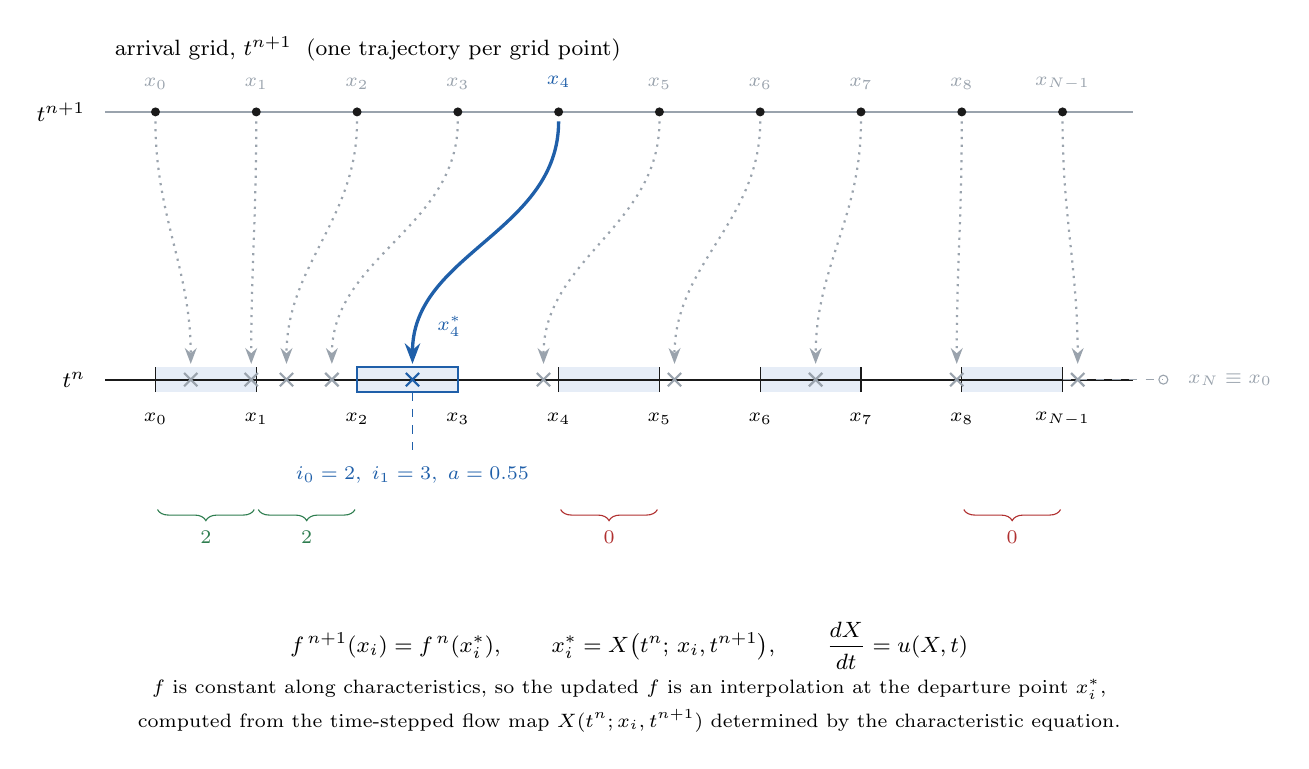
\begin{tikzpicture}[x=1.28cm,y=1cm]
  \foreach \k in {0,2,4,6,8} \fill[soft] (\k,-0.16) rectangle (\k+1,0.16);
  \draw[gridc,thick] (-0.5,3.4) -- (9.7,3.4);
  \draw[ink,thick] (-0.5,0) -- (9.7,0);
  \foreach \i in {0,...,9} \node[gpt] at (\i,3.4) {};
  \foreach \i/\lb in {0/0,1/1,2/2,3/3,5/5,6/6,7/7,8/8} \node[slbl,gridc] at (\i,3.76) {$x_{\lb}$};
  \node[slbl,accent] at (4,3.78) {$x_{4}$};
  \node[slbl,gridc] at (9,3.76) {$x_{N-1}$};
  \foreach \i in {0,...,9} {\draw[ink] (\i,-0.16) -- (\i,0.16);}
  \foreach \i/\lb in {0/0,1/1,2/2,3/3,4/4,5/5,6/6,7/7,8/8} \node[slbl] at (\i,-0.5) {$x_{\lb}$};
  \node[slbl] at (9,-0.5) {$x_{N-1}$};
  \node[ghost] at (10,0) {};
  \node[slbl,gridc,anchor=west] at (10.15,0) {$x_N\equiv x_0$};
  \draw[gridc,dashed] (9,0) -- (10,0);
  \foreach \i/\d in {0/0.35,1/0.95,2/1.30,3/1.75,5/3.85,6/5.15,7/6.55,8/7.95,9/9.15}{
    \draw[traj] (\i,3.28) to[out=-90,in=90] (\d,0.2);
    \node[dep,gridc] at (\d,0) {};
  }
  \draw[htraj] (4,3.28) to[out=-90,in=90] (2.55,0.2);
  \node[dep] at (2.55,0) {};
  \node[slbl,accent,anchor=west] at (2.70,0.68) {$x^{*}_{4}$};
  \draw[accent,thick] (2,-0.16) rectangle (3,0.16);
  \draw[accent,dashed] (2.55,-0.16) -- (2.55,-0.95);
  \node[slbl,accent,anchor=north] at (2.55,-0.98) {$i_0=2,\; i_1=3,\; a=0.55$};
  \node[lbl,anchor=west] at (-0.5,4.2) {arrival grid, $t^{n+1}$ \;(one trajectory per grid point)};
  \node[lbl,anchor=east] at (-0.6,0) {$t^{n}$};
  \node[lbl,anchor=east] at (-0.6,3.4) {$t^{n+1}$};
  \draw[decorate,decoration={brace,amplitude=4pt,mirror},good] (0.02,-1.65) -- (0.98,-1.65);
  \node[slbl,good] at (0.5,-2.0) {2};
  \draw[decorate,decoration={brace,amplitude=4pt,mirror},good] (1.02,-1.65) -- (1.98,-1.65);
  \node[slbl,good] at (1.5,-2.0) {2};
  \draw[decorate,decoration={brace,amplitude=4pt,mirror},bad] (4.02,-1.65) -- (4.98,-1.65);
  \node[slbl,bad] at (4.5,-2.0) {0};
  \draw[decorate,decoration={brace,amplitude=4pt,mirror},bad] (8.02,-1.65) -- (8.98,-1.65);
  \node[slbl,bad] at (8.5,-2.0) {0};
  \node[slbl,anchor=west] at (9.6,-2.0) {};
  \node[anchor=north,align=center] at (4.7,-2.95)
   {\footnotesize $\displaystyle f^{\,n+1}(x_i)=f^{\,n}(x^{*}_i),
    \qquad x^{*}_i=X\big(t^{n};\,x_i,t^{n+1}\big),
    \qquad \frac{dX}{dt}=u(X,t)$\\[3pt]
    \scriptsize $f$ is constant along characteristics, so the updated $f$ is an interpolation at the
    departure point $x^{*}_i$,\\
    \scriptsize computed from the time-stepped flow map $X(t^{n};x_i,t^{n+1})$ determined by the
    characteristic equation.};
\end{tikzpicture}
\end{document}
